\documentclass[border=10pt]{standalone}

\usepackage{tikz}
\usepackage{tikzsymbols}
\usetikzlibrary{calc,patterns,shapes.geometric}

\def\centerarc[#1](#2)(#3:#4:#5){\draw[#1] ($(#2)+({#5*cos(#3)},{#5*sin(#3)})$) arc (#3:#4:#5);}

\begin{document}
	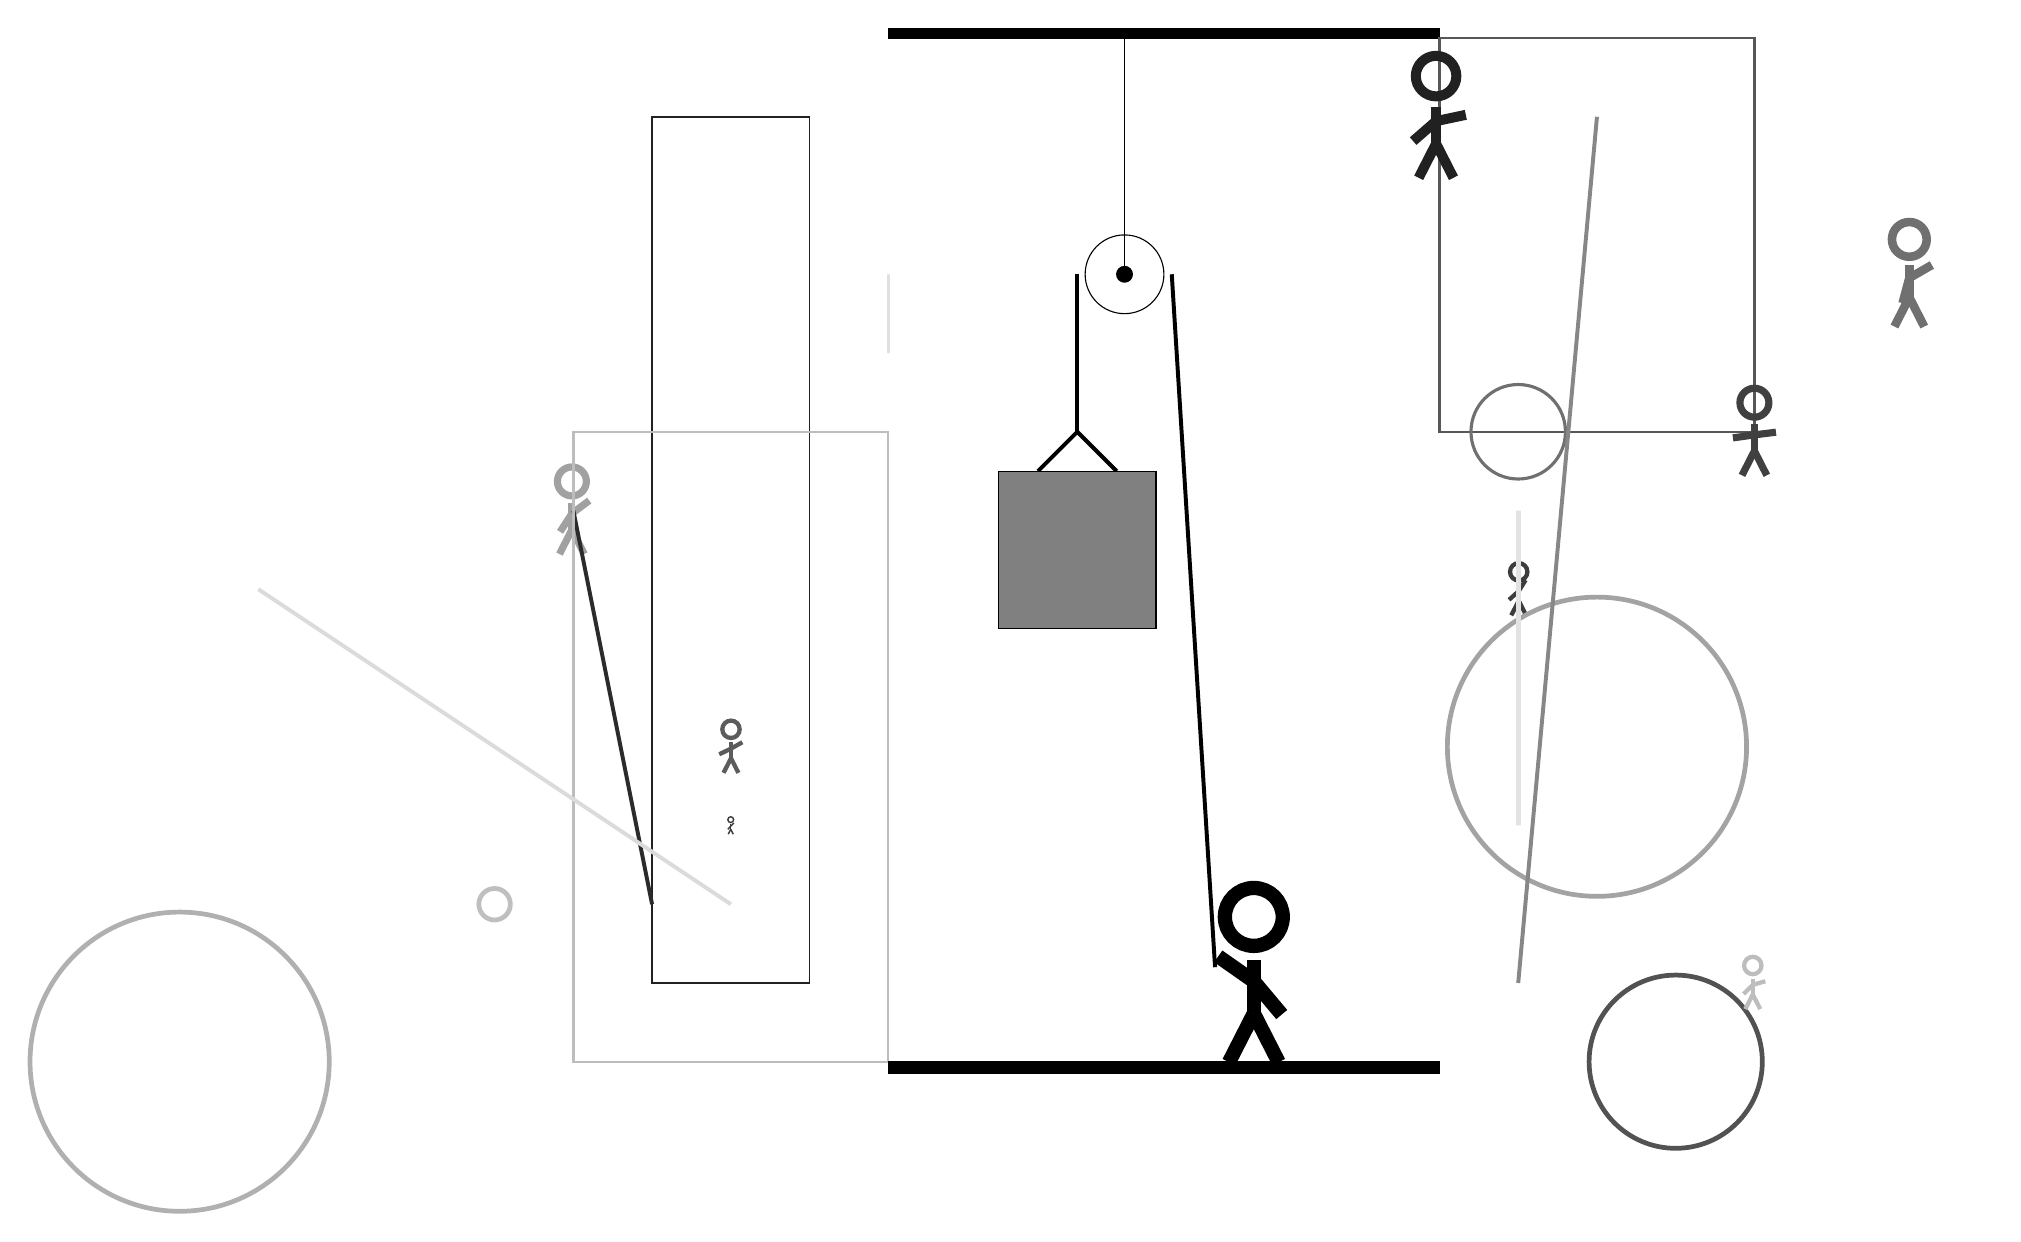
\begin{tikzpicture}
		%%%%% START %%%%%
		
		\draw[fill=black] (-2, 10) rectangle (5, 10.125);
		
		\draw (1, 7) circle (0.5);
		\draw[fill=black] (1, 7) circle (0.1);
		\draw (1, 10) -- (1, 7);
		
		\draw[line width=0.5mm] (-0.1, 4.5) -- (0.4, 5.0) -- (0.9, 4.5);
		\draw[fill=black!50] (-0.6, 4.5) rectangle (1.4, 2.5);
		
		\draw [line width=0.6mm, color=black!68](8, -3) circle (1.1);
		
		\draw [line width=0.6mm, color=black!86](-4, 3) circle (0.0);
		\node[line width=0.4mm, color=black!37] at (-6, 4) {\Strichmaxerl[5][57][37]};
		\draw[line width=0.2mm, color=black!87] (-3, -2) rectangle (-5, 9);
		\draw [line width=0.6mm, color=black!31](-11, -3) circle (1.9);
		\draw[line width=0.3mm, color=black!66] (5, 5) rectangle (9, 10);
		\draw[line width=0.5mm, color=black!83](-6, 4) -- (-5, -1);
		\node[line width=0.7mm, color=black!76] at (6, 3) {\Strichmaxerl[3][42][58]};
		\draw [line width=0.6mm, color=black!25](-7, -1) circle (0.2);
		
		\draw [line width=0.6mm, color=black!36](7, 1) circle (1.9);
		\draw[line width=0.3mm, color=black!26] (-2, -3) rectangle (-6, 5);
		\node[line width=0.7mm, color=black!75] at (9, 5) {\Strichmaxerl[5][8][7]};
		\node[line width=0.4mm, color=black!56] at (11, 7) {\Strichmaxerl[6][75][30]};
		
		\draw [line width=0.4mm, color=black!56](6, 5) circle (0.6);
		\draw[line width=0.5mm, color=black!47](6, -2) -- (7, 9);
		\draw[line width=0.4mm, color=black!12] (-2, 7) rectangle (-2, 6);
		\draw[line width=0.5mm, color=black!14](-4, -1) -- (-10, 3);
		\node[line width=0.3mm, color=black!64] at (-4, 1) {\Strichmaxerl[3][26][29]};
		\draw[line width=0.6mm, color=black!11] (6, 4) rectangle (6, 0);
		
		\node[line width=0.4mm, color=black!26] at (9, -2) {\Strichmaxerl[3][45][16]};
		\node[line width=0.3mm, color=black!77] at (-4, 0) {\Strichmaxerl[1][48][45]};
		\draw [line width=0.5mm, color=black!49](12, 8) circle (0.0);
		\node[line width=0.7mm, color=black!87] at (5, 9) {\Strichmaxerl[7][41][12]};
		
		\draw[line width=0.5mm] (0.4, 7) -- (0.4, 5.0);
		\centerarc[line width=0.5mm](1, 7)(0:180:0.6);
		\draw[line width=0.5mm](1.6, 7) -- (2.15, -1.8);
		
		\node at (2.6, -1.9) {\Strichmaxerl[10][-35][-50]};
		
		\draw[fill=black] (-2, -3) rectangle (5, -3.15);
		
		%%%%% END %%%%%
	\end{tikzpicture}
\end{document}